\documentclass[conference]{IEEEtran}
\IEEEoverridecommandlockouts
% The preceding line is only needed to identify funding in the first footnote. If that is unneeded, please comment it out.
\usepackage{cite}
\usepackage{amsmath,amssymb,amsfonts}
\usepackage{algorithmic}
\usepackage{graphicx}
\usepackage{textcomp}
\usepackage{xcolor}
\usepackage{listings}
\lstset{captionpos=b,basicstyle=\footnotesize}

\graphicspath{{../figures/}}
\def\BibTeX{{\rm B\kern-.05em{\sc i\kern-.025em b}\kern-.08em
    T\kern-.1667em\lower.7ex\hbox{E}\kern-.125emX}}
\begin{document}


\title{Disabling Prefetcher to Enhance Cache Side Channels}

\author{\IEEEauthorblockN{1\textsuperscript{st} Meet Udeshi}
\IEEEauthorblockA{\textit{Electrical Engineering Department} \\
\textit{Indian Institute of Technology, Bombay}}
}

\maketitle

\begin{abstract}
Cache side channels are well known for being effective
in extracting data from modern cryptographic ciphers.
Side channel attacks gather data on their own cache hits and cache misses,
and can infer the program's memory accesses based on this data.
Such attacks assume that the victim program is the only other one making accesses
to the shared cache. Any accesses not originating from the victim program
lead to false positives which introduces noise in the side channel.
Attackers can restrict other programs from running on the core and
synchronize the attack with execution of relevant section of code of the
victim program. However, they cannot directly switch off hardware units
like Prefetchers which may generate accesses to the cache.
This work describes a method in which the prefetcher is prevented
from generating any accesses using an attack tailored to disable its
function.
\end{abstract}

\begin{IEEEkeywords}
security, side channels, prefetcher
\end{IEEEkeywords}

\section{Introduction}

 % Side channels look at cache accesses of victim to deduce data
An attacker program using the cache as a side channel tries to force
collisions with the victim program by making accesses which alias to the
same cache lines \cite{osvik-cache-attacks}.
Time taken for subsequent accesses to these cache lines differs and is used to
determine whether there was a successful collision or not.
This data is further used to infer whether the victim accessed a particular
cache line or not, thus leaking data about the data of the program.
 % Prime+Probe determines if victim evicted certain cache set
 % when it's own data is evicted from that cache set. It looks for
 % cache miss.
Different implementations of the side channel look for either a cache
hit or a cache miss as a sign of successful collision.
The Prime+Probe attack fills the cache lines in a set with data other than
that being accessed by the victim. Any access by the victim to that set will
cause attacke's data to be evicted, which will show up during the Probe step
as a cache miss \cite{osvik-cache-attacks}.
 % Flush+Reload tries to get a cache hit on the data victim may have
 % accessed, like a common library.
Similarly, the Flush+Reload attack looks for a cache hit to the same
data as the victim. A cache hit in the Reload step is infered as successful
collision \cite{percival-rsa}.

 % Side channel attacks require least interference, else they will get
 % false positives because an attacker cannot determine where the cache
 % access came from.
 % They can only deduce properly if correct code segment of
 % program is executing, nobody else.
 % Any other entity accessing the cache will interfere
The attacker assumes a scenario where only the victim is making memory
accesses, hence is able to deduce the memory access pattern. If there is
another program or hardware making memory accesses, they will surely
interfere with the side channel. After obtaining a successful collision,
there is no way for the attacker to distinguish whether the source of
this collision was truly the victim. Fuchs et al \cite{fuchs-disruptive}
introduce a Disruptive Prefetcher which generates spurious memory accesses,
making the victim's accesses indistinguishable for any attacker.

 % To reduce interference of prefetcher we try to disable the prefetcher
This paper focuses on a way to disable the prefetcher and significantly reduce
the number of generated prefetches. With a separate attacker focusing on disabling
the prefetcher, it becomes extremely unlikely for the side channel attacker to
see a collision with a prefetcher generated access. This enhances the side channel
and can enable faster and better data retrieval.
 % Work focuses on stride prefetcher but it can be extended to
 % any PC-indexed prefetcher or buffer based prefetcher.
The attack implementation has been designed specific to a Stride prefetcher
\cite{fu-stride}. However, the implementation can be used as-is or easily extended
to apply to any PC-indexed prefetcher table.

 % Stride prefetcher trains on stride value for a certain PC by storing
 % a confidence counter. Disabling prefetcher involves not letting
 % it train on PC values.
 % Some more detail on working of stride prefetcher
A Stride Prefetcher tries to identify certain load instructions which have
a memory access pattern

\section{Attack Vectors}

 - Prefetcher will be disabled when it does not get to the condition
   of generating prefetches.
 - They generate prefetch when confidence value crosses threshold.
 - Confidence value is reset below threshold when a new entry is made to the table.
   This is exploited by periodically making new entries into the table
   to evict older entries and prevent them from gaining confidence.
 - This attack vector allows us to never let victim's load instruction
   trigger the prefetcher to generate prefetches.
 - Confidence is decremented when an entry hits in the table and the stride
   value does not match. Attacker randomises the stride value in every access.
 - This prevents attacker from generating any prefetches
   which would be detrimental to the purpose.
 - Prefetcher is only accessed when there is a cache miss, clflush instruction is
   used to always generate a cache miss.

\section{Attacker Implementation}

 - To add new entries to Prefetcher table, we need to have a load
   instruction at new location.
 - A binary is created which contains large number of
   load instructions placed at different PC addresses so
   that after aliasing every entry of the prefetcher table is
   accessed atleast once.

\subsection{Full Attacker}

 - To make load instructions alias to every entry, their PC addresses
   need to be carefully controlled. The set indexing bits need
   to attain every possible value enough times to fill all ways.
 - Single load is 4 bytes in X86. accompanying clflush is 3 bytes.
   sequence of 7 bytes placed one after other will skip certain
   set indexes. A particular set index may have many loads aliasing
   to it while another may have very few.
 - To properly control, padding with nop instruction is required.
 - Describe why 8 byte sequence and sequence length + nop

\begin{lstlisting}[caption={Full Attacker disassembly: load misses at different PCs},
label={lst:full_attack}]
00000000000006ca <attack>:
 6ce: 8b 58 36     mov    0x36(%rax),%ebx
 6d1: 90           nop
 6d2: 0f ae 78 36  clflush 0x36(%rax)
 6d6: 8b 58 08     mov    0x8(%rax),%ebx
 6d9: 90           nop
 6da: 0f ae 78 08  clflush 0x8(%rax)
 6de: 8b 58 3f     mov    0x3f(%rax),%ebx
 6e1: 90           nop
 6e2: 0f ae 78 3f  clflush 0x3f(%rax)
 6e6: 8b 58 38     mov    0x38(%rax),%ebx
 6e9: 90           nop
 6ea: 0f ae 78 38  clflush 0x38(%rax)
 6ee: 8b 58 20     mov    0x20(%rax),%ebx
 6f1: 90           nop
\end{lstlisting}

 - This is called the full attacker because it targets the
   entire prefetcher table.
 - The full attacker takes time to run a single iteration of the attack
   because of the repeated cache misses and it contains ~256 loads.
 - It is possible (and also observed) that some load addresses of the victim
   can retrain the prefetcher while one iteration is running and generate
   prefetches.
 - These retrained load instructions will only be evicted in the next iteration.

\subsection{Targeted Attacker}
 - A faster implementation is required which can quickly evict notorious loads
   of the victim.
 - If such loads are identified in advance, an attacker which targets the
   sets of only such loads will be required.
 - Loads can be identified by looking at memory access patterns of the victim
   program by running simulations with multple random inputs.
 - From the full attacker we can leave relevant load instructions which
   alias with the targeted PCs, filter out others by replacing them with nop.
 - for targeting 2 PCs the number of load instructions required reduces from 256 to 16

\begin{lstlisting}[caption={Targeted attacker disassembly: loads at aliased PCs},
label={lst:targeted_attack}]
00000000000006ca <attack>:
     ...
 6d9: 90           nop
 6da: 8b 58 0f     mov    0xf(%rax),%ebx
 6dd: 0f ae 78 0f  clflush 0xf(%rax)
 6e1: 90           nop
 6e2: 90           nop
 6e3: 90           nop
 6e4: 8b 58 3c     mov    0x3c(%rax),%ebx
 6e7: 0f ae 78 3c  clflush 0x3c(%rax)
 6eb: 90           nop
 6ec: 90           nop
     <nop slide> ...
 6f7: 90           nop
 6f8: 8b 58 2f     mov    0x2f(%rax),%ebx
 6fb: 0f ae 78 2f  clflush 0x2f(%rax)
 6ff: 90           nop
     ...
\end{lstlisting}

 - The nop slides although important do not add any significant delay
   compared to the cache misses of load instructions.

\section{Simulation}

\begin{figure}[htbp]
    \centering
    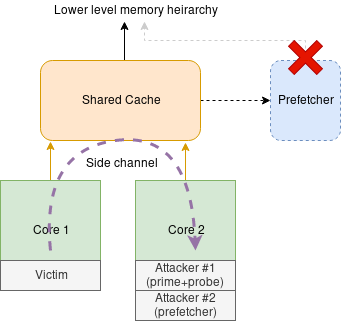
\includegraphics[width=\columnwidth]{prefetch_attack}
    \caption{Setup of attack to disable prefetcher from generating memory accesses}
    \label{fig:prefetch_setup}
\end{figure}

 - Gem5 X86 simulator
 - Two OoO cores with shared L2 cache
 - Stride prefetcher attached to L2 cache 16x4
 - Victim program runs on core 1 and attacker runs on core 2
 - Simulator measures number of prefetches issued, average confidence,
   hits and misses to table
 - These are measured for every 1 million instructions


\begin{table}
\centering
\begin{tabular}{|l|r|}
    \hline
    Simulator  & gem5 X86\\
    \hline
    Cores  & 2\\
    \hline
    L1 Icache & 32K 8-way\\
    \hline
    L1 Dcache & 32K 8-way\\
    \hline
    L2 cache & 256K 16-way shared between cores\\
    \hline
    L2 prefetcher  & Stride 64-entry 4-way, confthresh 4\\
    \hline
\end{tabular}
\\
\caption{Simulation setup}
\label{tab:simulation_setup}
\end{table}

\section{Results}

\begin{figure}[htbp]
    \centering
    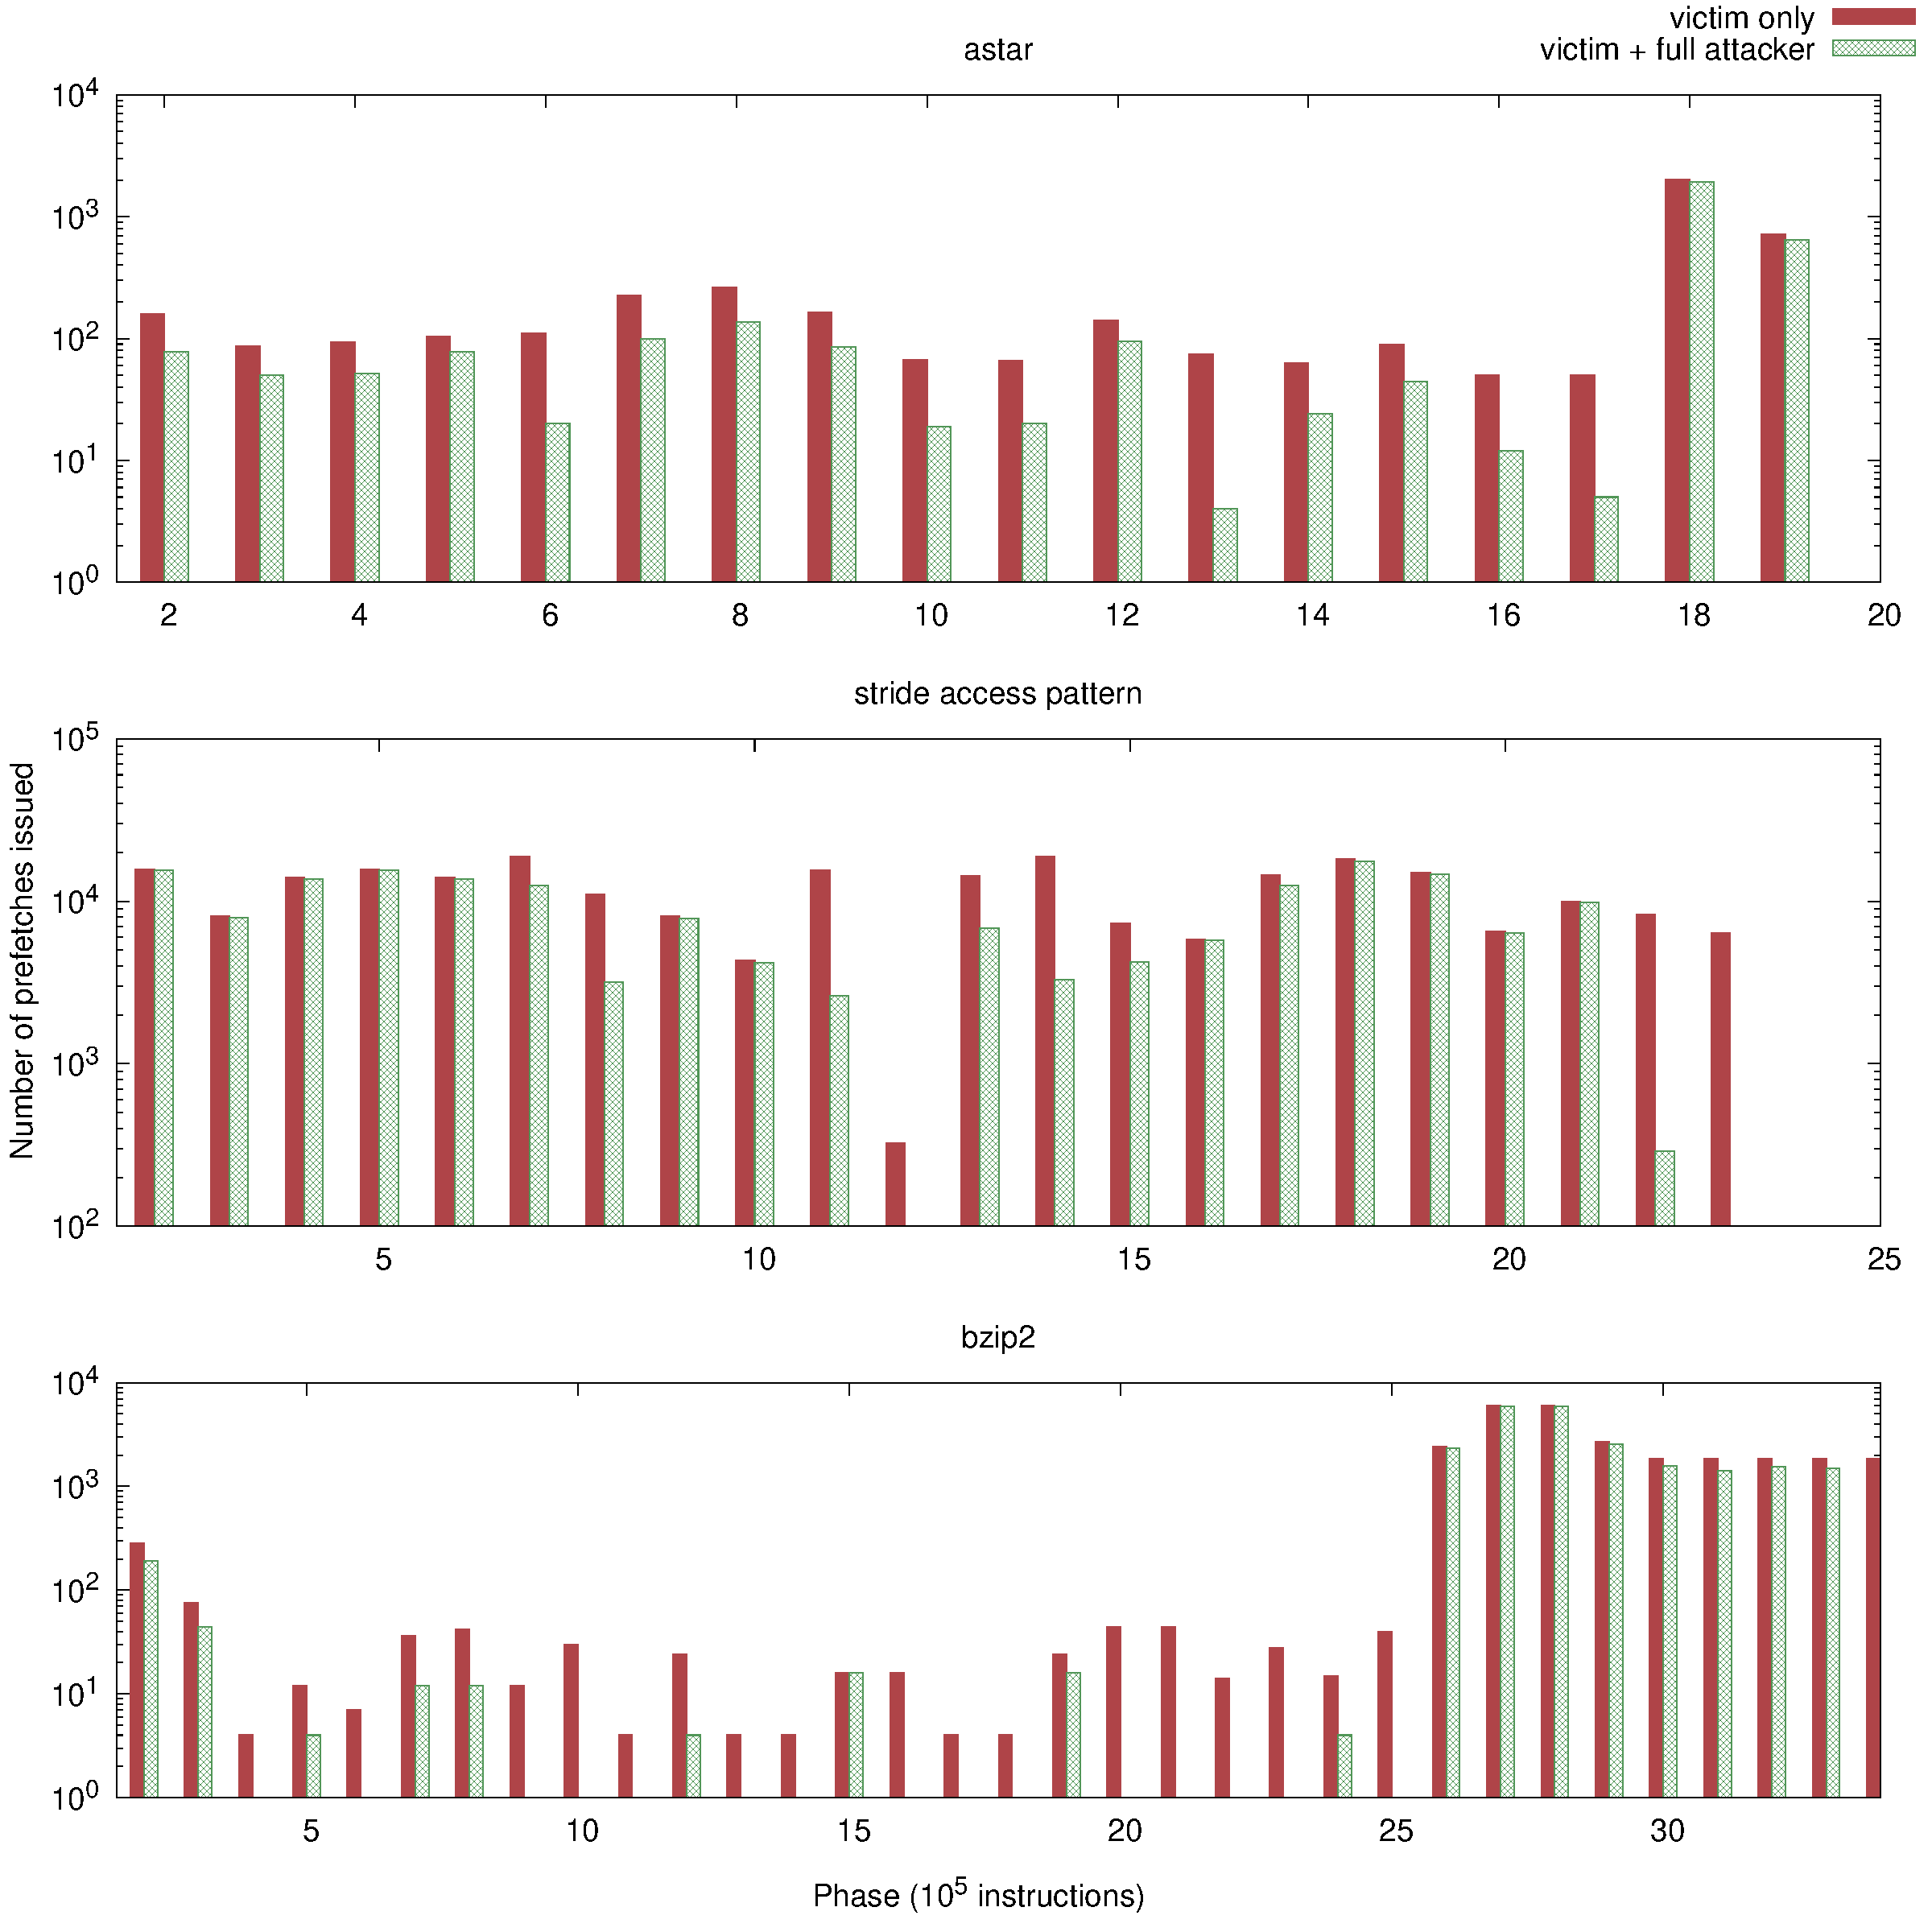
\includegraphics[width=\columnwidth]{hwpf_num}
    \caption{Number of prefetches issued on different benchmarks}
    \label{fig:prefetch_attack}
\end{figure}

\begin{figure}[htbp]
    \centering
    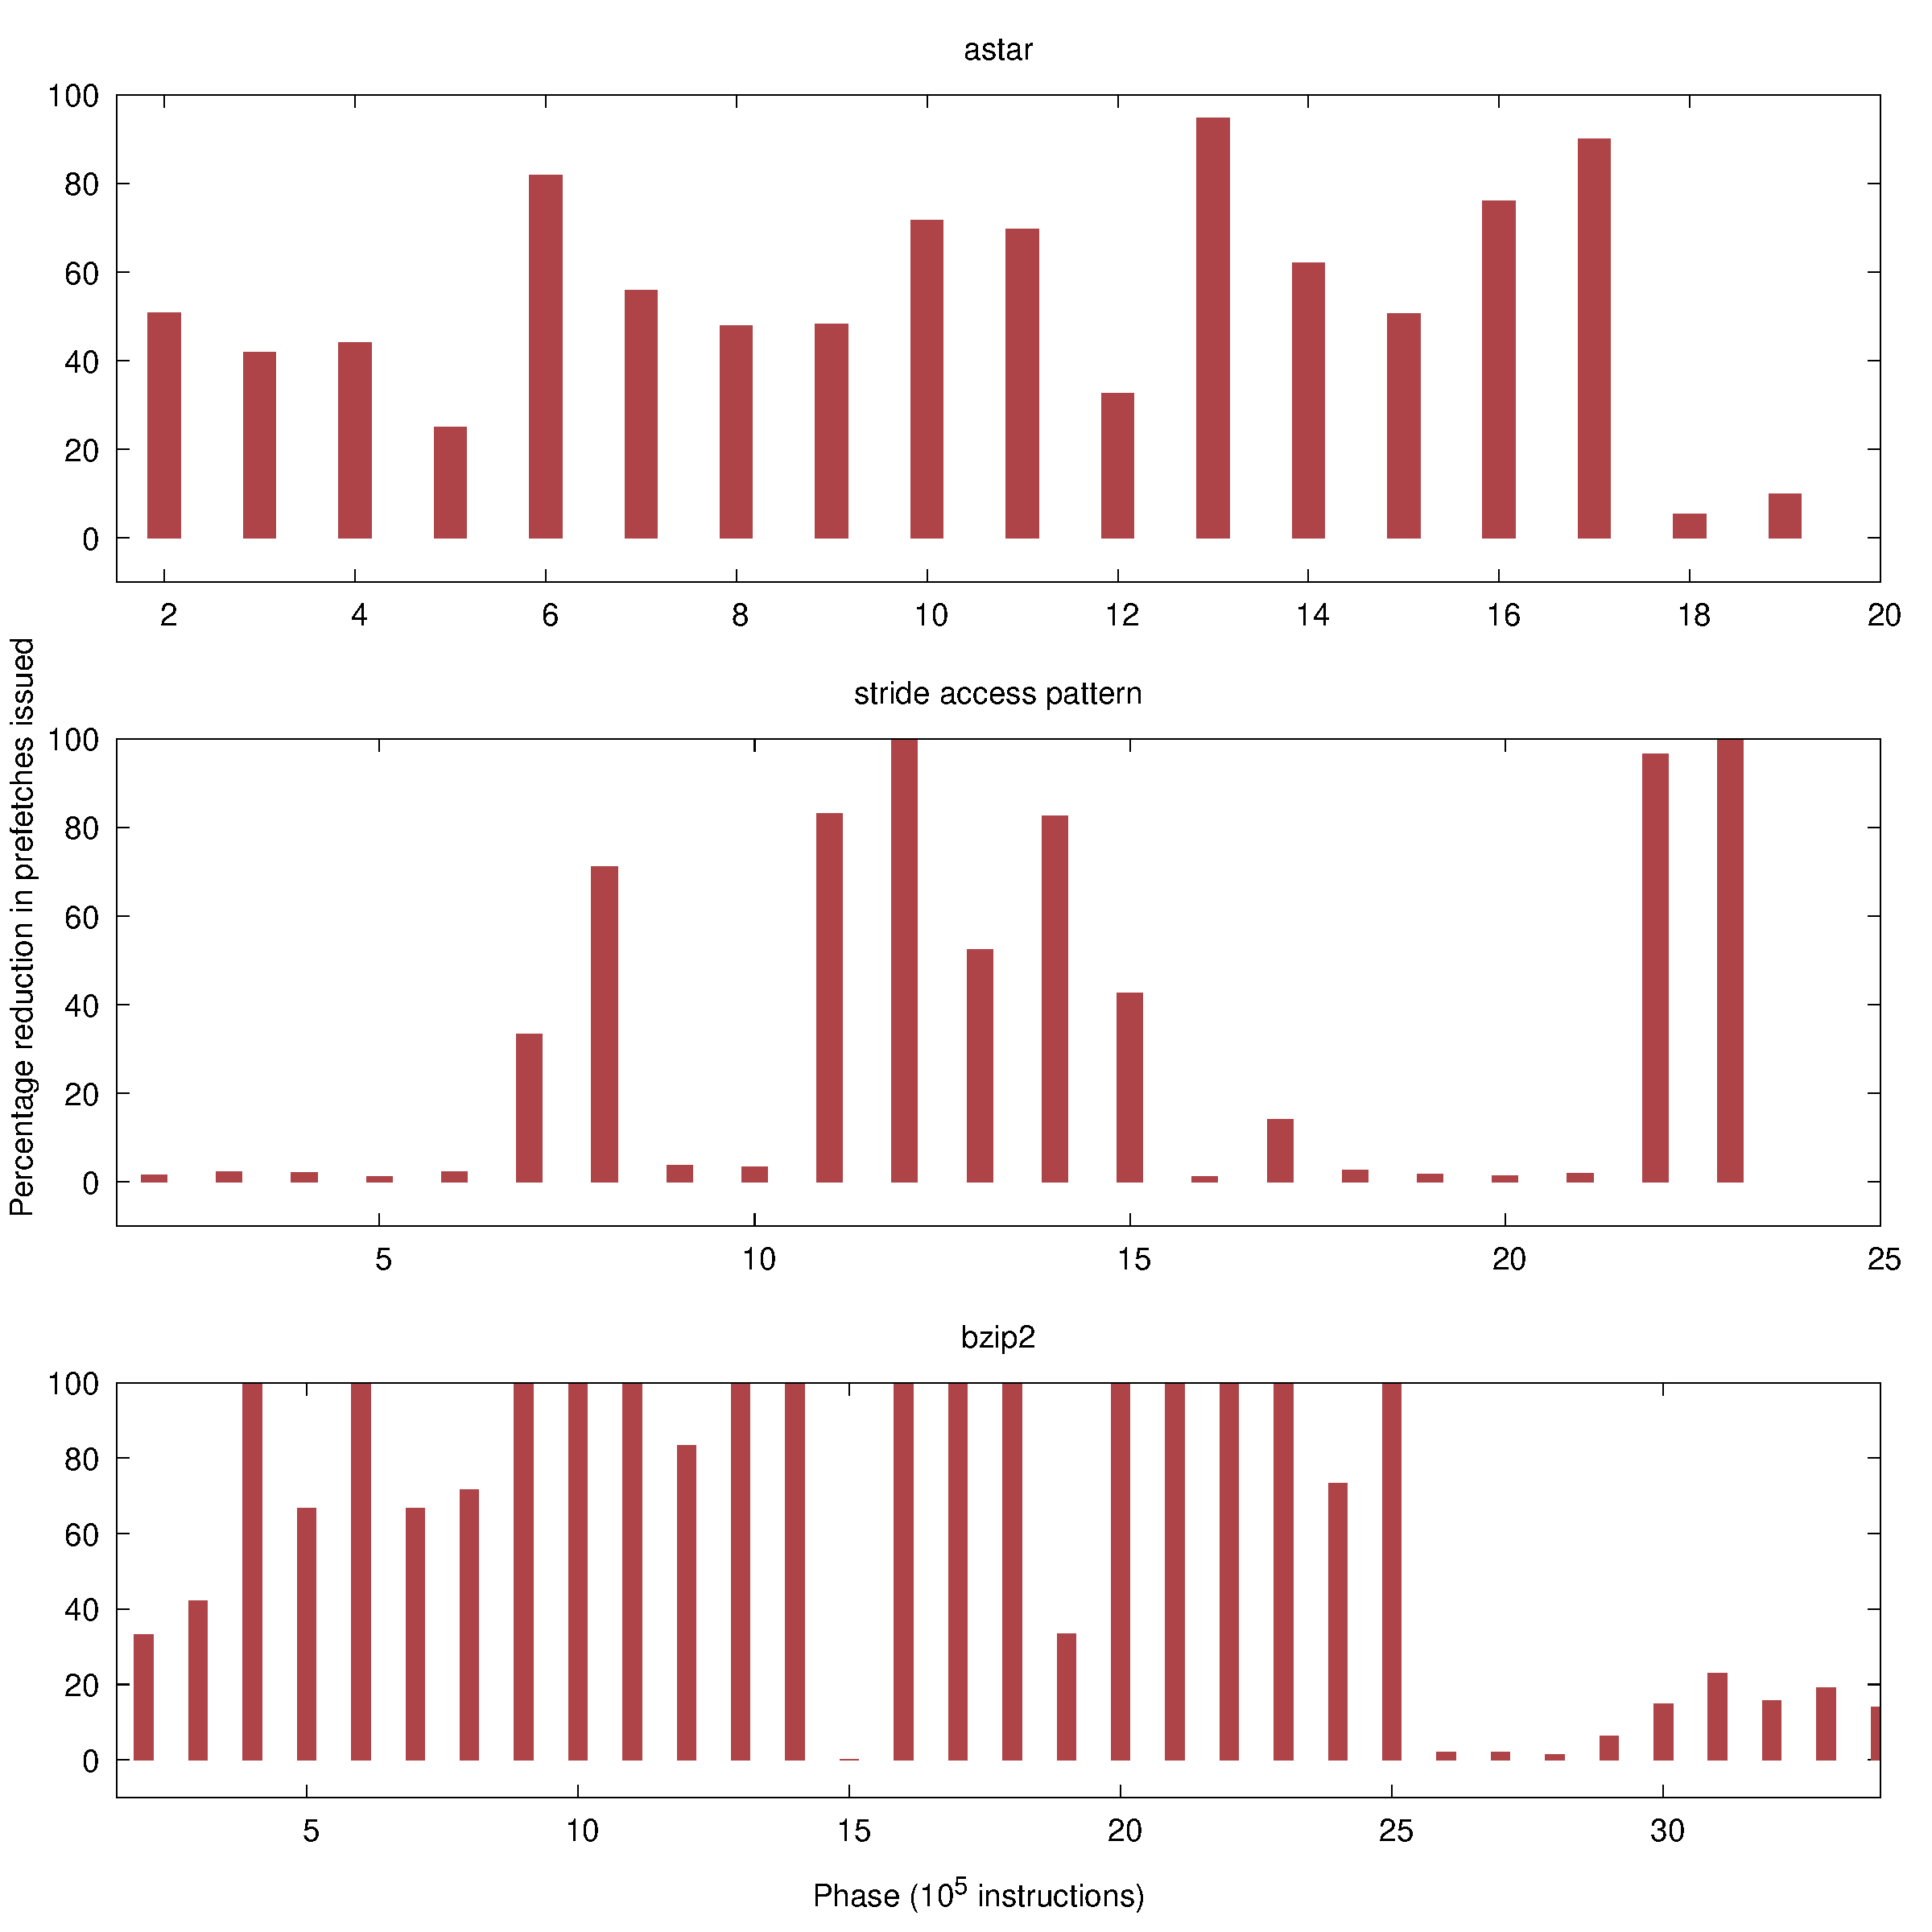
\includegraphics[width=\columnwidth]{hwpf_perc}
    \caption{Percentage reduction in number of prefetches}
    \label{fig:prefetch_percred}
\end{figure}

 - Benchmarks show full attacker is effective against some types of memory access
   patterns while others are not reduced much.

\begin{figure}[htbp]
    \centering
    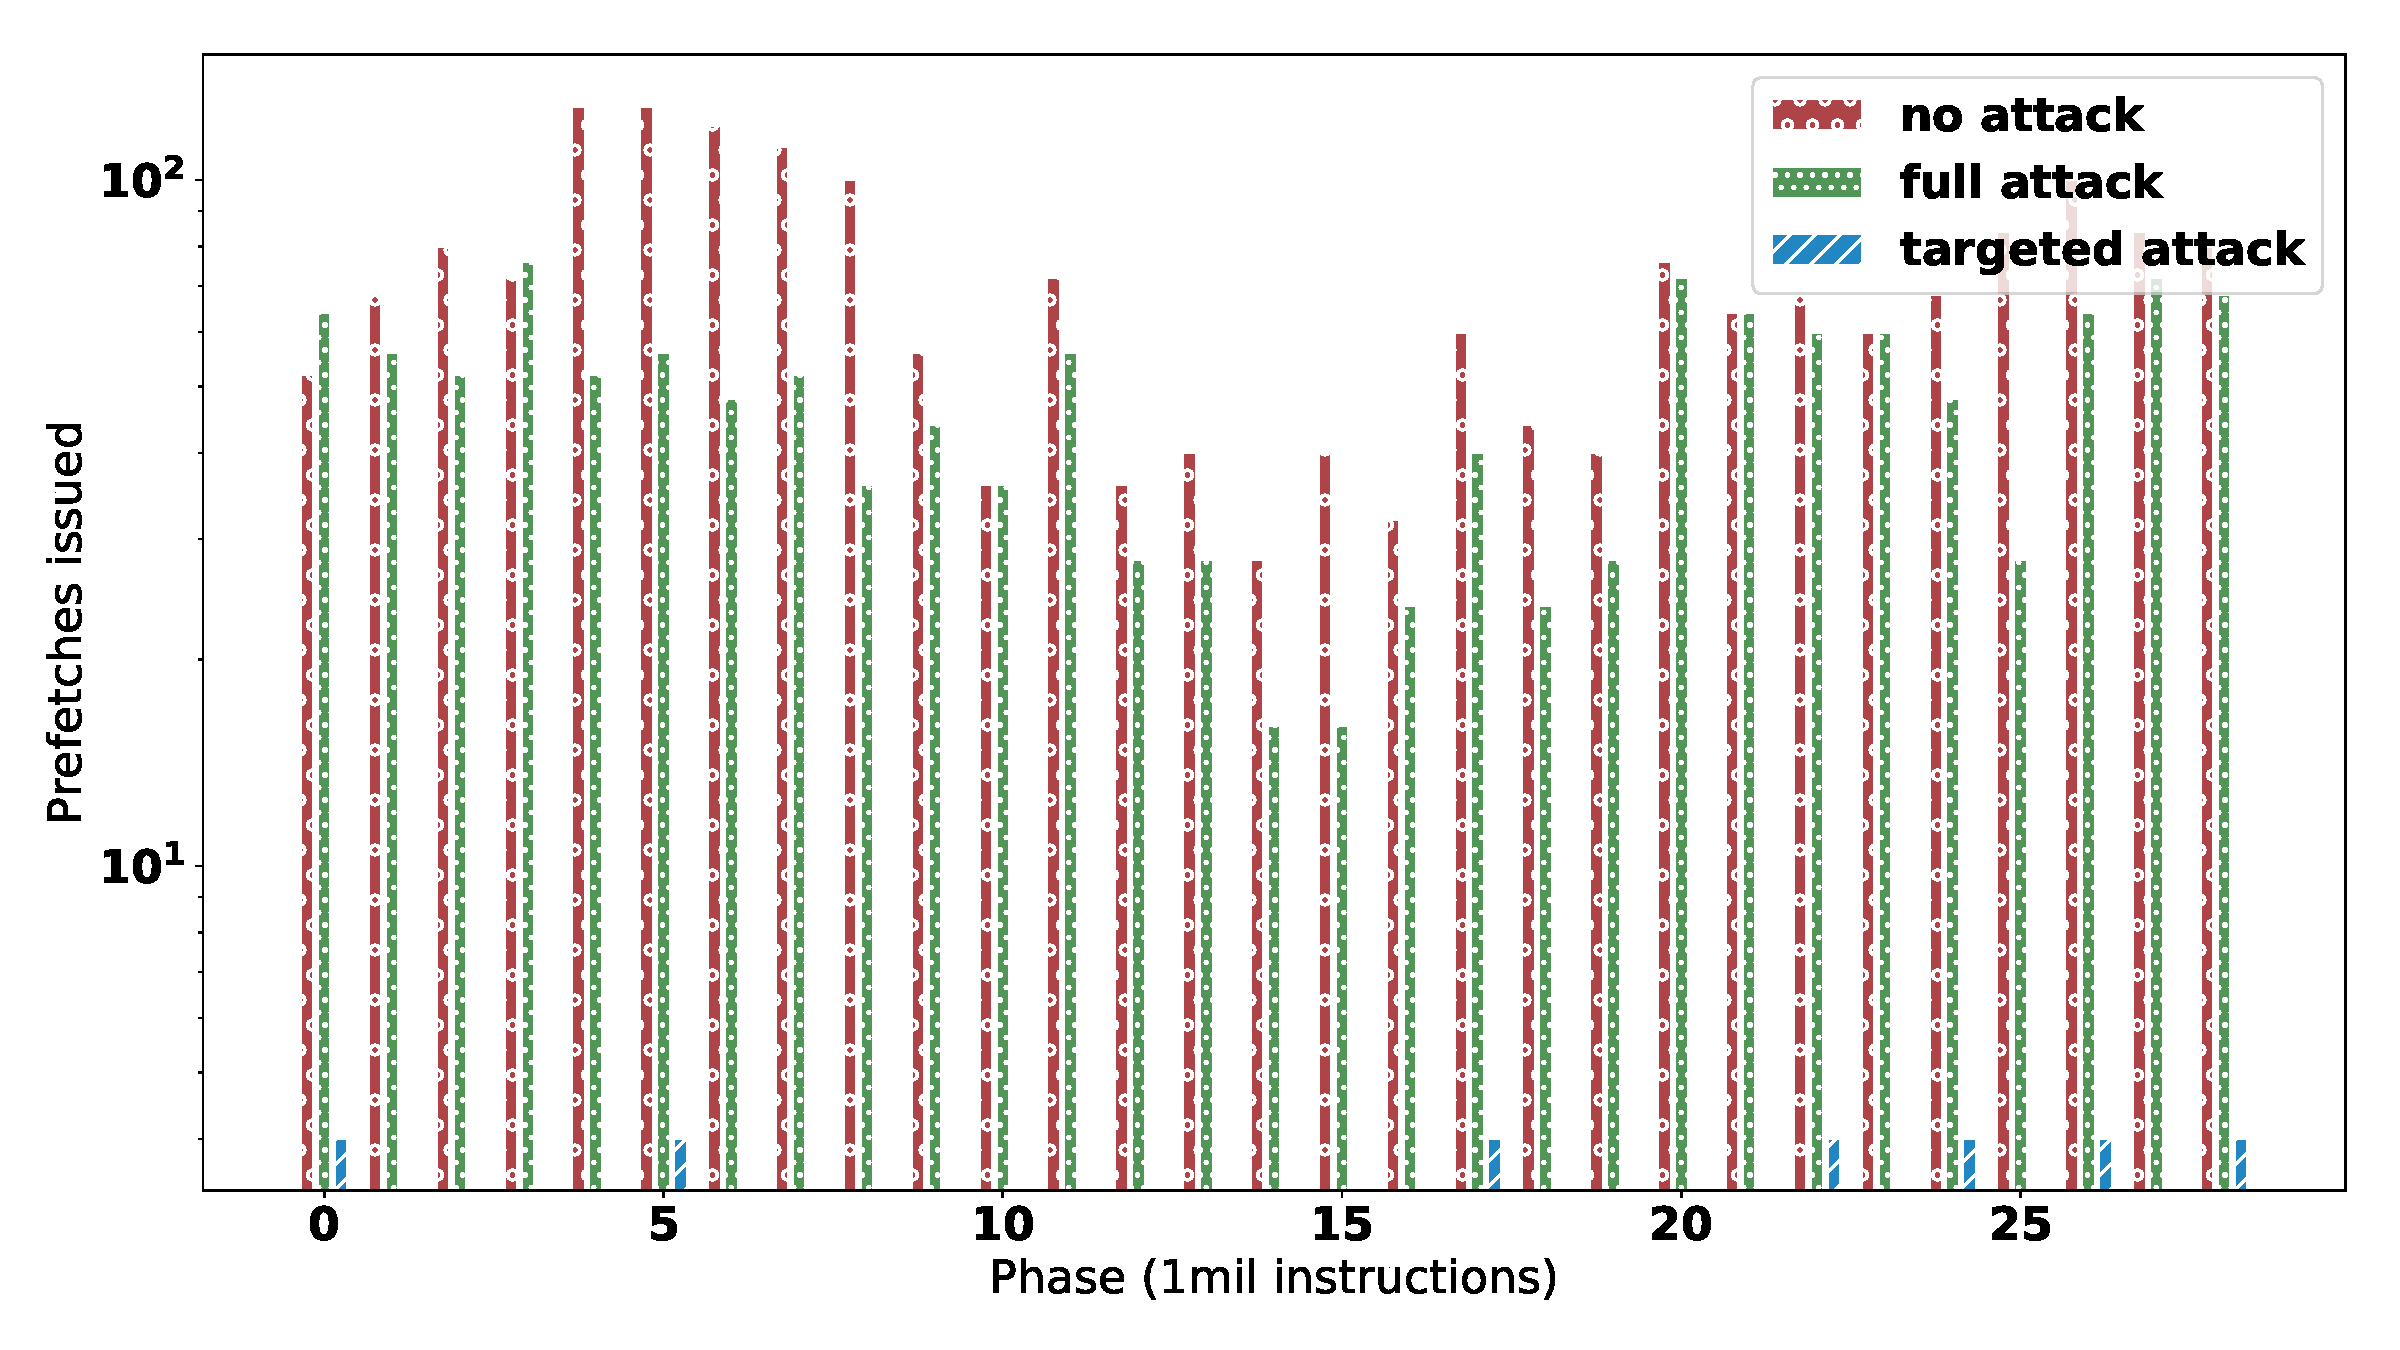
\includegraphics[width=\columnwidth]{pf_issued}
    \caption{Comparision of number of prefetches issued by AES program}
    \label{fig:targeted_attack}
\end{figure}

 - AES victim is implemented which encrypts random data using AES implementation
   of openssl 0.9.x (uses libcrypto)
 - Simulation of only victim helps identify two load addresses which generate
   most of the prefetches.
 - Targeted attacker is tailored to those load PCs
 - Full attacker is somewhat effective at reducing prefetches is some phases,
   but targeted attacker is extremely effective.

\begin{figure}[htbp]
    \centering
    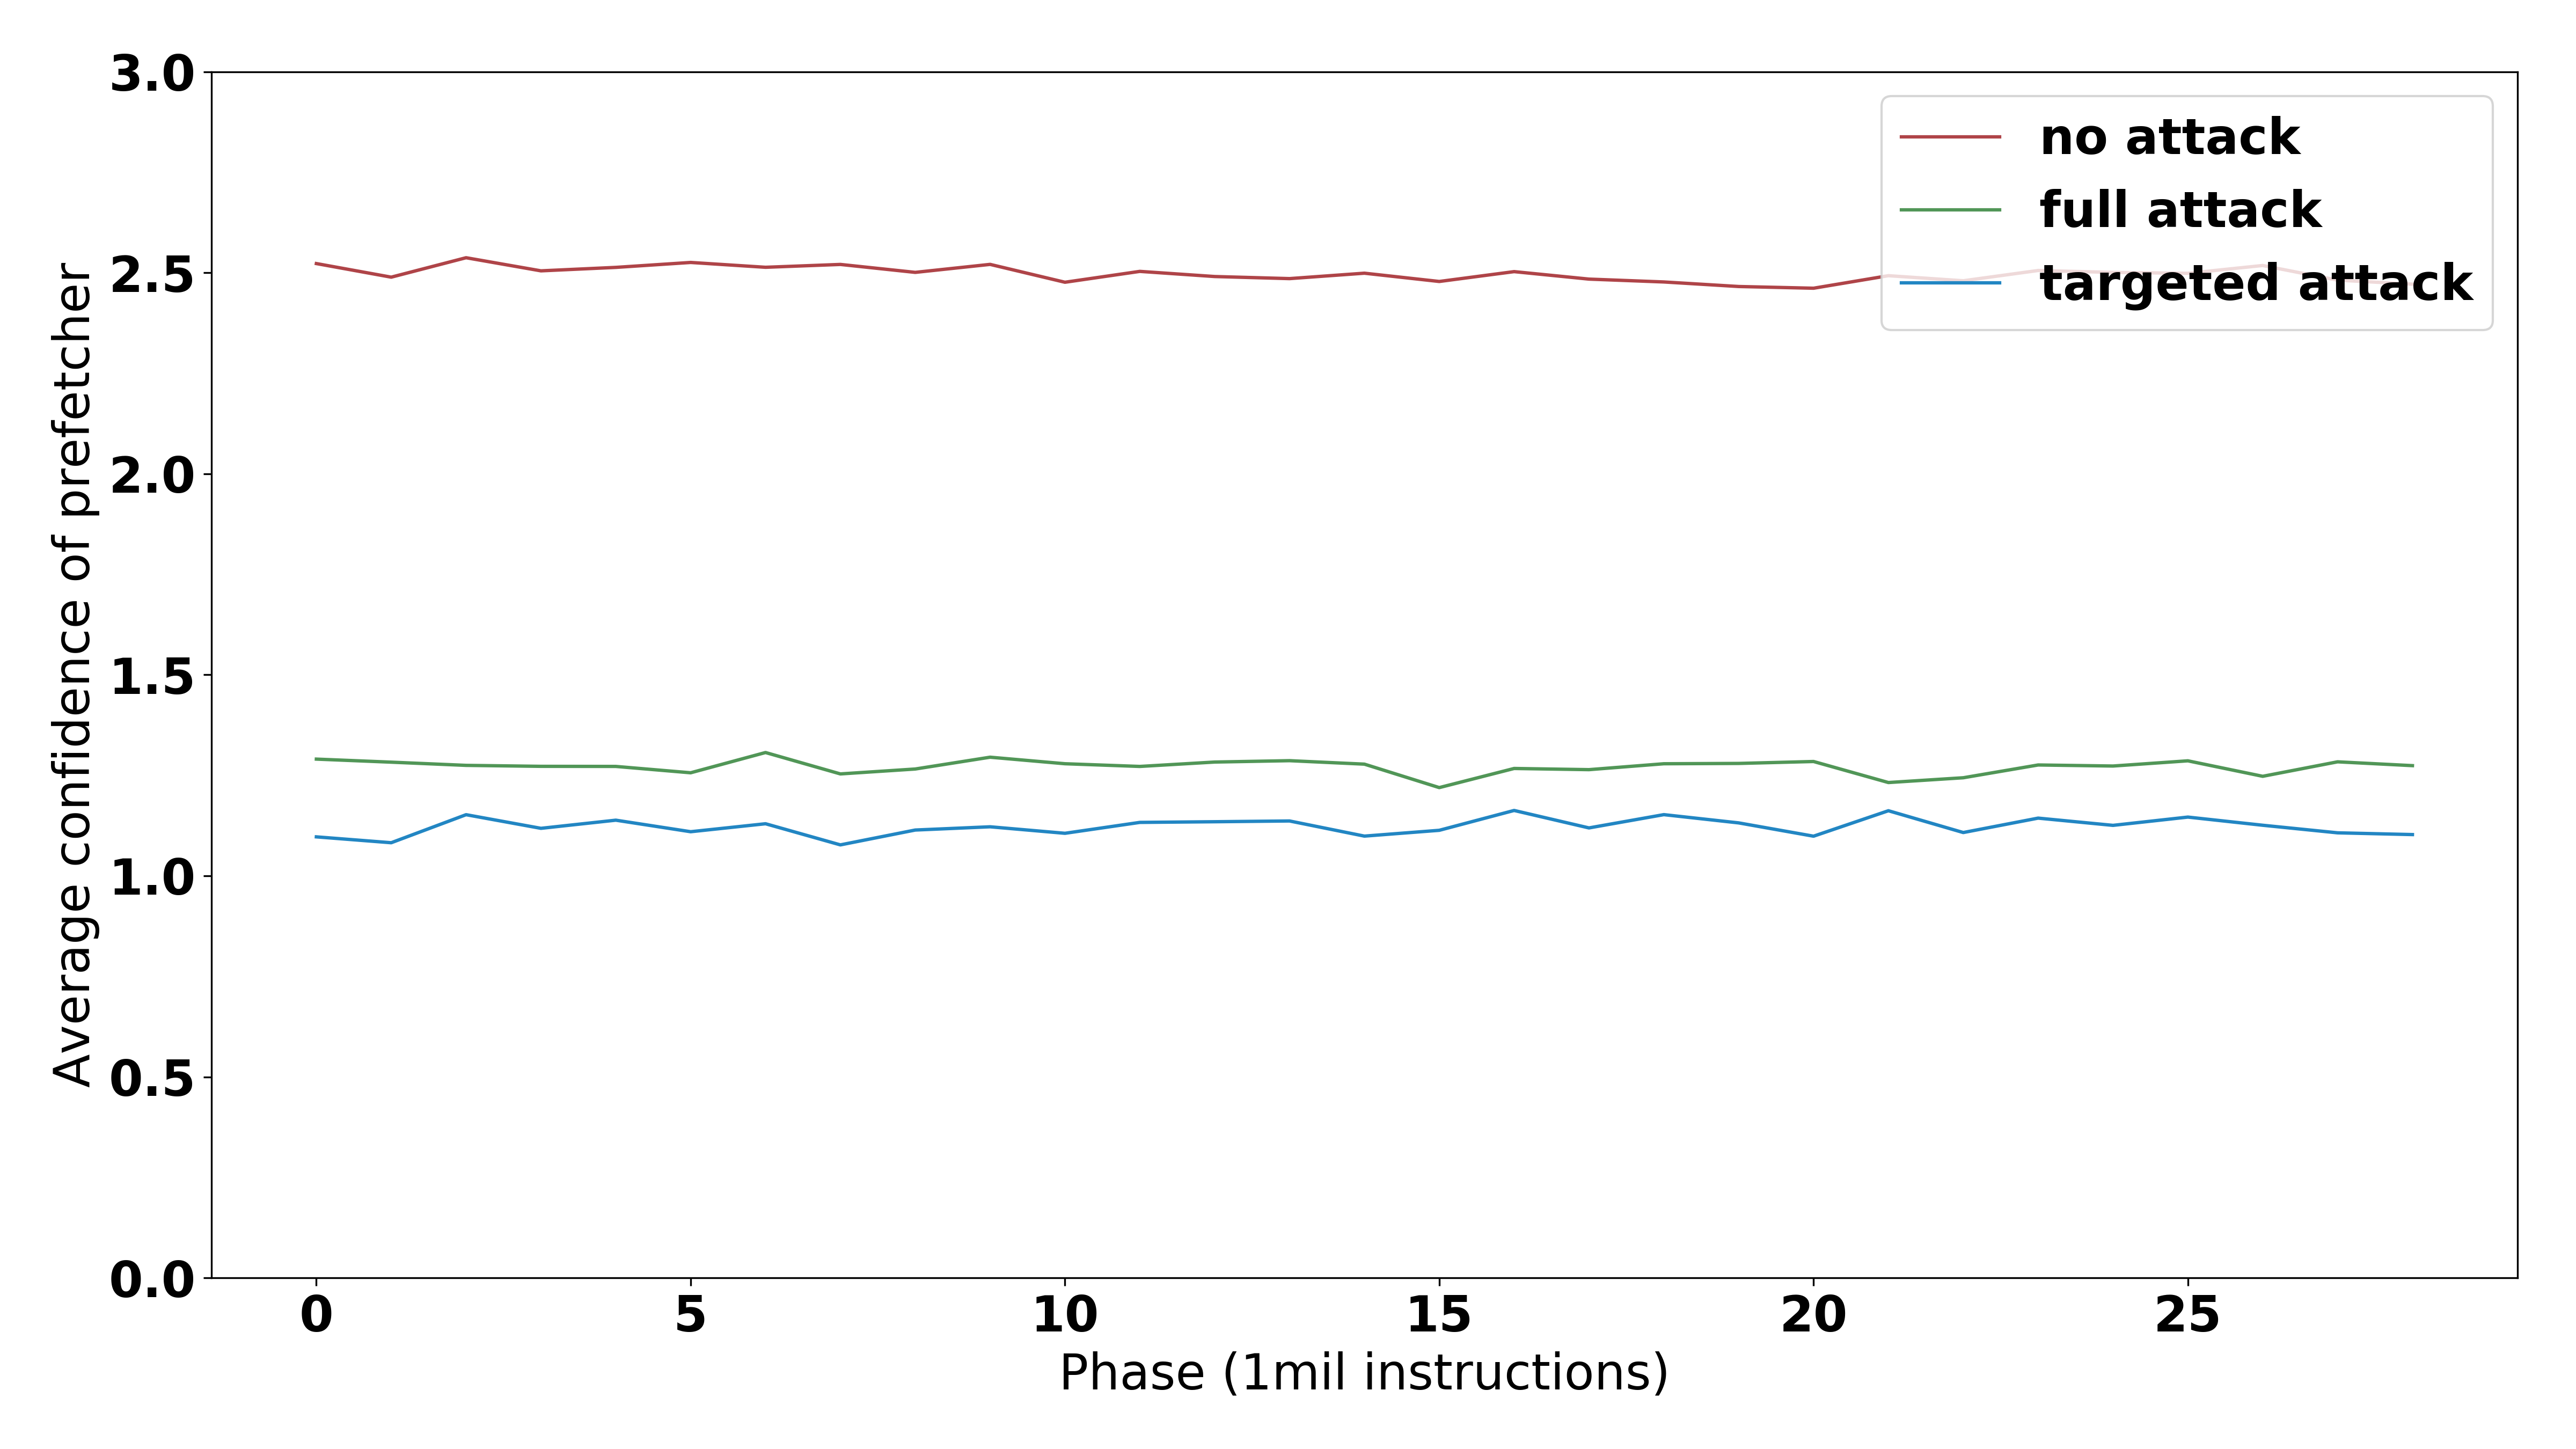
\includegraphics[width=\columnwidth]{avg_conf}
    \caption{Comparision of average confidence of prefetcher with AES program}
    \label{fig:targeted_avgconf}
\end{figure}

 - The targeted attacker and full attacker are able to equally reduce confidence
   of prefetcher

\begin{figure}[htbp]
    \centering
    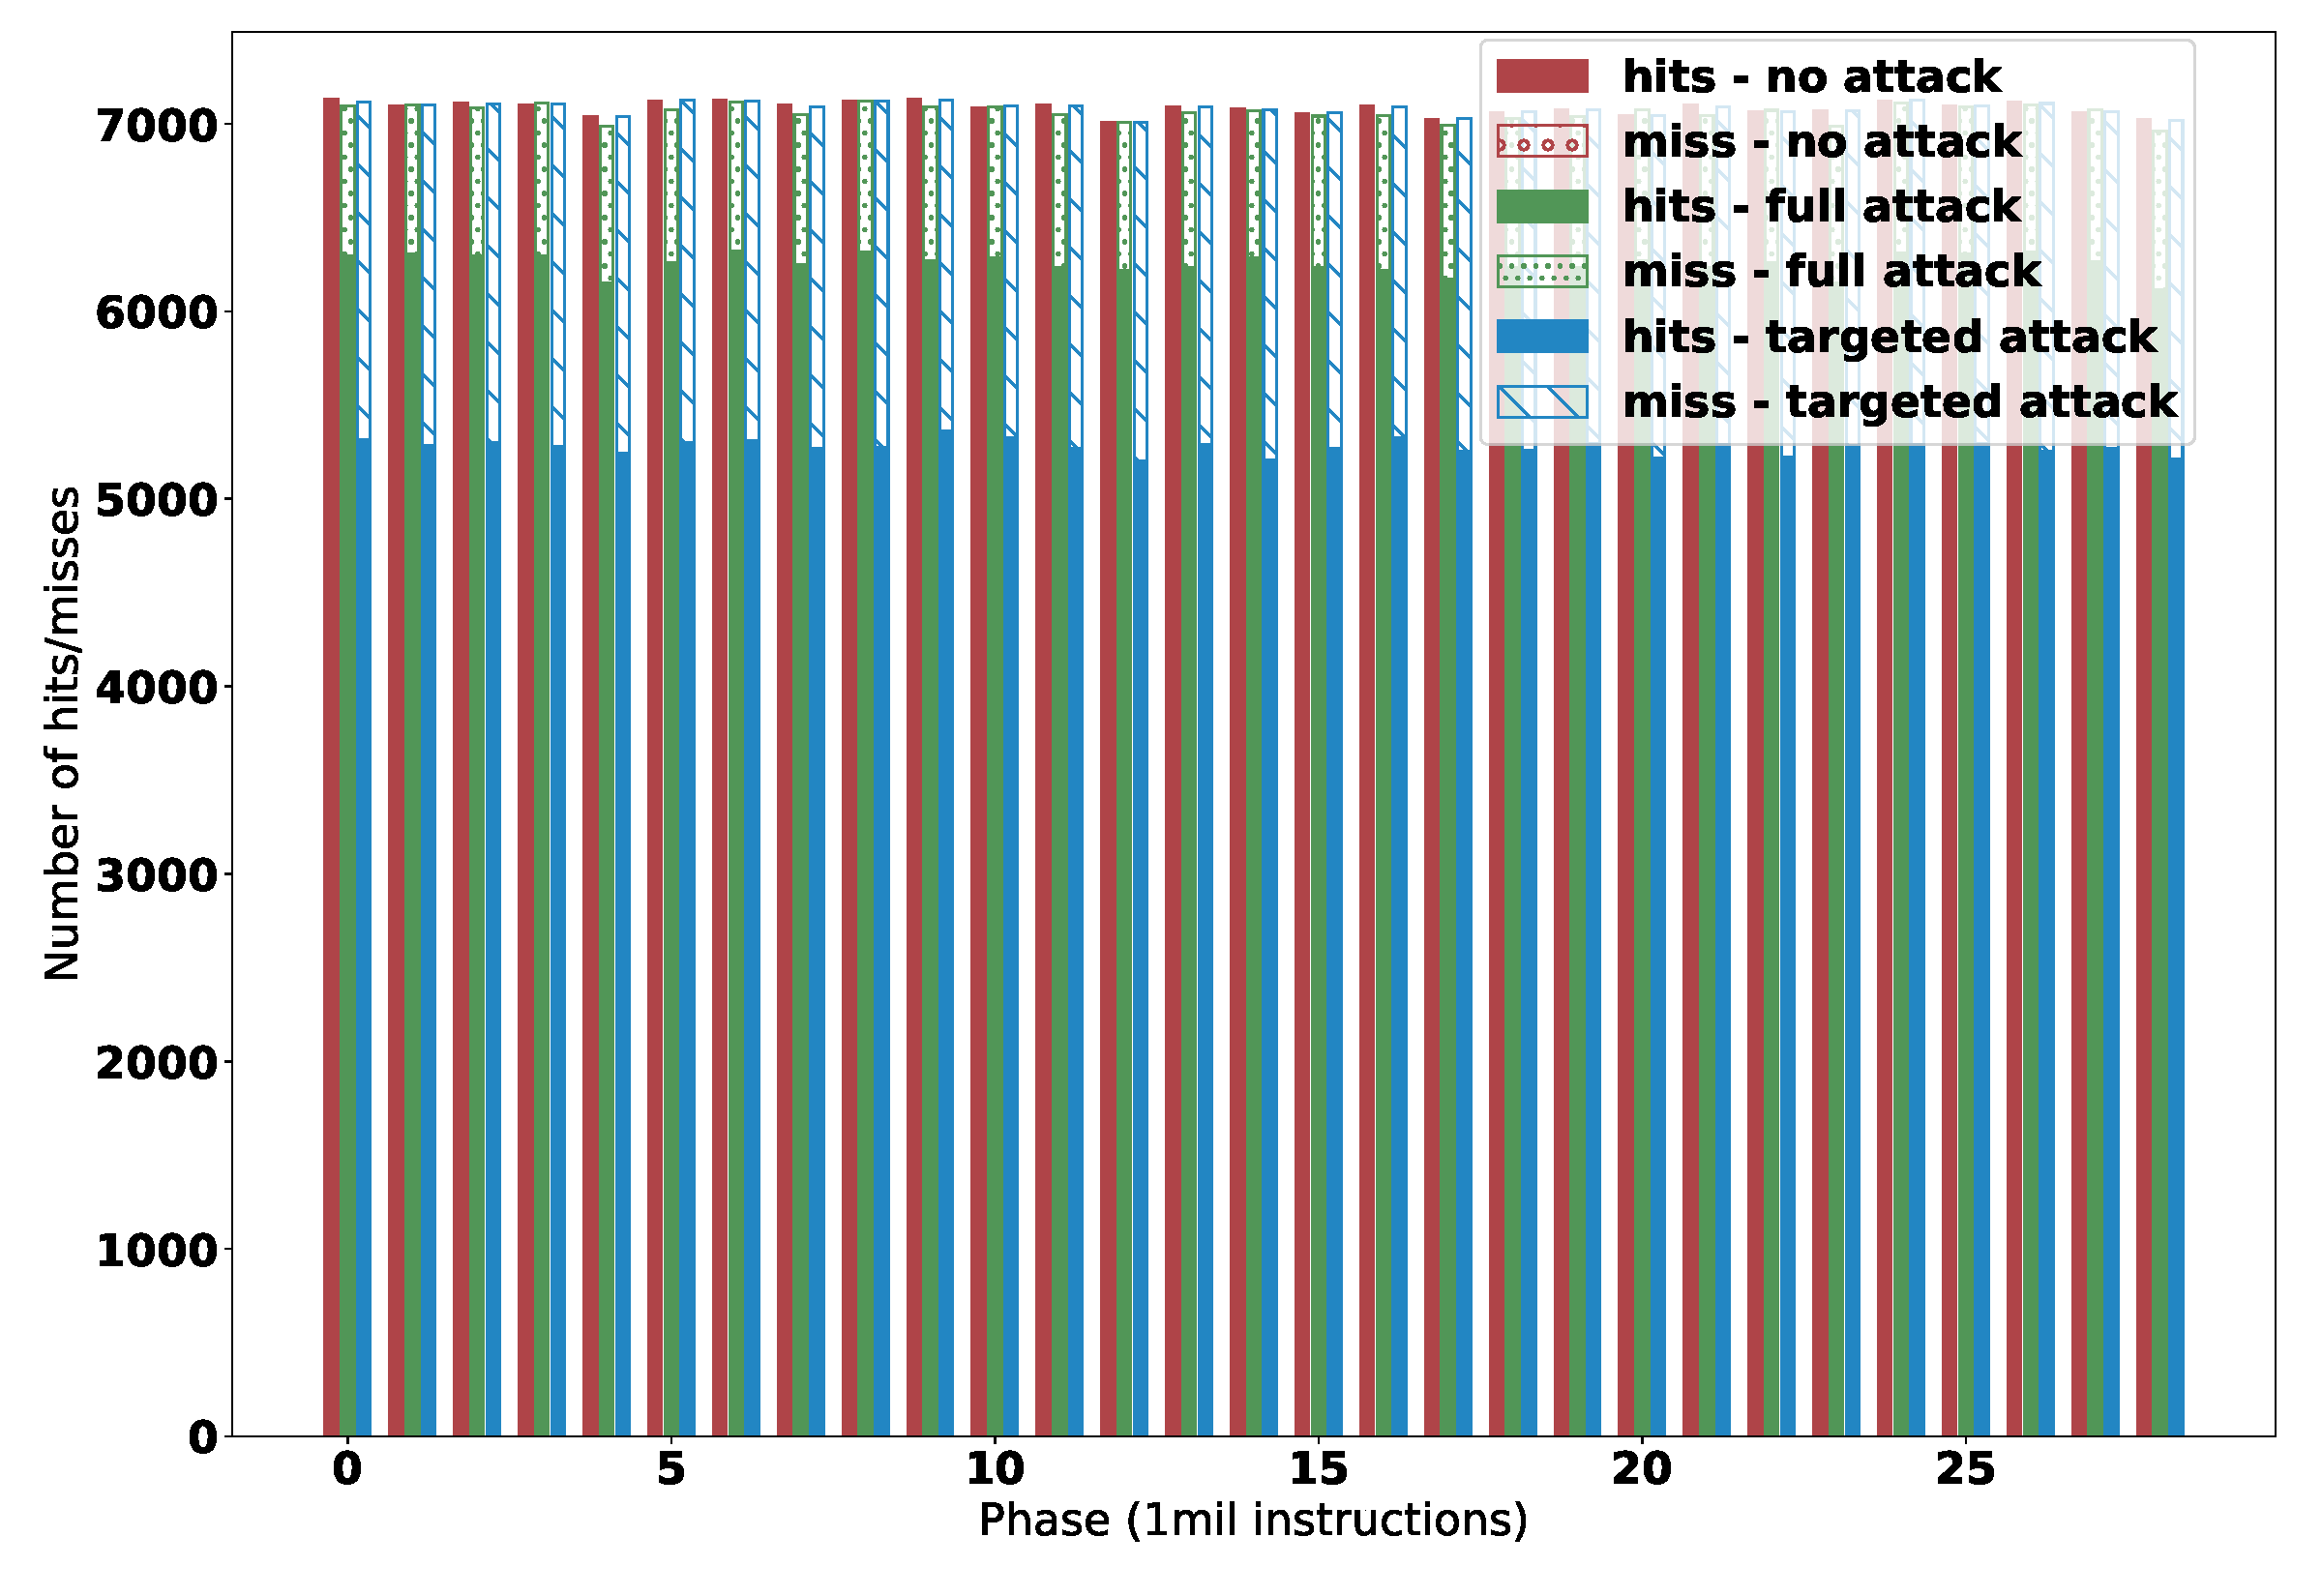
\includegraphics[width=\columnwidth]{pf_hits}
    \caption{Comparision of prefetch table hit and miss count by AES program}
    \label{fig:targeted_hitrate}
\end{figure}


 - Number of hits are significantly lower for targeted

DCPT prefetcher (hwpf)

 - Same implementation works very well for DCPT.
 - Full attacker works better, why ?

\section{Conclusion}

%\section*{Acknowledgment}

%\section*{References}

%\begin{thebibliography}{00}
%\end{thebibliography}
\bibliography{main}
\bibliographystyle{ieeetr}

\end{document}
